\chapter{Scan Agents}\label{sec:scan-agents}

\section{Overview}

Scan Agents are used as a method of performing some pre-scan processing of code to be submitted
for scan.  It can be considered similar to scripting that executes prior to submitting a scan
if executing in a CI/CD pipeline but with a much smaller scope of capabilities.  This is not
intended to replace the use of a CI/CD pipeline, but can assist with performing some basic
pre-scan steps for scans orchestrated by webhook events.

Performing pre-scan steps with the Scan Agent is similar to the mechanism of a CI/CD runner
used with SCMs that support integration of CI/CD pipelines.  An agent is installed on
a an existing runner agent or a standalone system, given a tag name that is representative
of the tooling environment, and is configured to receive scan requests from \cxoneflow.
The tooling environment tag is then referenced in the \cxone project configuration by
adding a tag to one or more project settings.


\section{Scan Agent Deployment}

Figure \ref{fig:scan-agent-deployment-diagram} shows a deployment diagram for some typical
Scan Agent deployment types.  The top box shows the Scan Agent process running on the same
machine as the CI/CD runner.  This is often a better way to perform a deployment given the
runner will typically have the correct development tooling installed and properly maintained
over time.  The bottom box shows the Scan Agent deployed on the "Build Box" that would have
similar properties as the CI/CD runner but may use other methods to invoke builds.


\begin{figure}[ht]
  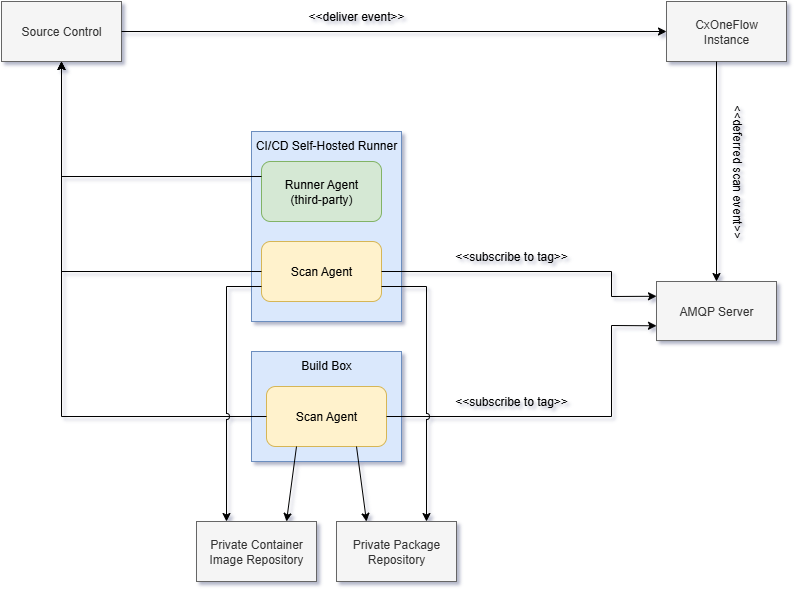
\includegraphics[width=\textwidth]{graphics/cxoneflow-diagrams-Scan Agent Diagram.png}
  \caption{Scan Agent Deployment Diagram}
  \label{fig:scan-agent-deployment-diagram}
\end{figure}


\subsection{Scan Agent Security Considerations}\label{sec:scan-agent-security-considerations}

Performing code builds, as is typically performed in a CI/CD pipeline, often includes
a bit of risk in that a build requires the execution of scripting.  There are often
controls in place to prevent anyone other than trusted authors from authoring the build scripts.
If those controls fail or are bypassed, the Scan Agent could be made to execute arbitrary
script commands which could include executing attacker-controlled code.

The use of Scan Agents involves some of the same risks as those that exist in
CI/CD pipeline builds.  The pre-scan scripting is controlled by the
administrator that is deploying the Scan Agent; this can help to limit the exposure
of arbitrary shell script execution.  Schemes where the script detects and executes
additional commands that are provided by code from the repository can create
a remote code execution attack vector.  If the use of the pre-scan scripting is designed
to execute commands found in the code under scan, use caution.

Executing \scaresolver can also represent a remote code execution attack vector when the package manager has
the capability for the package resolution to execute code.  A package manifest,
usually provided by code checked into the repository, that references a malicious package may also
open a remote code execution attack vector.  The scope of what can be accomplished by a malicious package
executing in the build system will depend on what the malicious package is allowed to execute and what data
it can exfiltrate from a system where it is executing.

The deployment details in the following sections will provide security recommendations
that, if followed, can minimize the impact if Scan Agents' execution
capabilities are somehow exploited.  Scenarios where \scaresolver and the pre-scan script are executed in
an instance of a container can limit the impact of any exploits but should not be expected
to completely avoid all potential impacts. 

The \cxoneflow endpoint server itself does not invoke any scripting or tools as part of the 
Scan Agent workflow; this action is delegated to the Scan Agents.  However, be aware that a required step of the
Scan Agent execution is to obtain a clone of the code for scanning.  To facilitate this,
the \cxoneflow endpoint server does send encoded SCM credentials to authorized
Scan Agents.  Section \ref{sec:scan-agent-security} has more details
about security considerations for Scan Agent installation.

The purpose of the \scaresolver scan is to detect vulnerable and malicious packages. It
should therefore be anticipated that malicious packages may be inadvertently referenced
by developers in the package manifest.  If the step to execute \scaresolver is enabled
and the package manifest references a malicious package, take all precautions that
would be suitable to assess anything that may have been modified by any actions the package
manager allowed the malicious package to execute.

The following security recommendations should be considered as part of deployment of \cxoneflow with Scan Agents:
\begin{itemize}
  \item Use SSL for all message queue connections.
  \item Use SSL connections for delivering SCM events to the \cxoneflow endpoints.
  \item Isolate the Scan Agent either through installing on isolated subnets or using OS permissions to
  isolate the Scan Agent runtime.
  \item Configure Scan Agents to execute build tools inside containers to isolate the \scaresolver and pre-scan execution from
  the Scan Agents' runtime.
  \item If a scan detects a malicious package, rotate all credentials used by \cxoneflow and Scan Agents
  after the reference to the malicious package is removed from the source code.\footnote{CAUTION: Opening the code that
  references a malicious package in an IDE may also execute the package's malicious payload!}
\end{itemize}

\section{Server Configuration for Scan Agents}\label{sec:scan-agent-server}

Implementing the Scan Agents requires an AMQP message queue server that
is used for communication between the \cxoneflow server and the Scan
Agents.  Details about the message queue deployment can be found in Section \ref{sec:external-mq}.

The examples in this section show a configuration that uses environments names as tags to
instruct the Scan Agents with that environment tag to perform pre-scan and \scaresolver
execution.  The tags names can be used to establish the Scan Agent affinity with \cxone projects
in whatever way fits your organization best.

\subsection{\cxoneflowtext\space Endpoint Configuration}

The \cxoneflow endpoint server \intlink{sec:yaml-config}{YAML configuration} will not utilize Scan Agents
by default.  Using Scan Agents requires a public/private key pair; the private key is configured
for use on the \cxoneflow endpoint and the public key is installed with each Scan Agent.  Before
configuring the use of Scan Agents, it is recommended to read about the security
concepts in Section \ref{sec:scan-agent-security}.

The \cxoneflow endpoint will send messages signed by the private key to the Scan
Agents using the message queue.  The receiving Scan Agent will validate the signature
using the public key; if the signature is not valid, the Scan Agent will reject the message
and perform no actions.

Scan Agents are identified using agent tags.  The \cxoneflow endpoint is configured by the
administrator with a list of allowed tags to prevent arbitrary Scan Agents from requesting
scan activity delegation.  The server-side tag configuration is also used to set up the communication
with Scan Agents via the message queue.  Anyone who installs a Scan Agent must configure it to respond to messages
targeting at least one valid Scan Agent tag.


\subsubsection{Generating a Public/Private Key Pair}\label{ref:server-key-pair}

There are many ways to generate a public/private key pair.  There are only a few requirements
for key pairs produced by any method:

\begin{itemize}
  \item The private key must be unencrypted.
  \item Both the private and public key files must be PEM encoded.
  \item The public/private key algorithm is supported by the install Python \texttt{cryptography} library.
    As of this release, these algorithms have been tested:
  \begin{itemize}
      \item RSA 4096-bit
      \item ECDSA secp256k1
  \end{itemize}
\end{itemize}

One easy method of generating a public/private key pair is to use OpenSSL.  To generate an ECDSA public/private key pair,
the following command can be used.  The command will create the file \texttt{ec-priv.pem} that holds the unencrypted private key
and the file \texttt{ec-pub.pem} that holds the public key.

\begin{code}{OpenSSL Public/Private Key Creation}{[ECDSA]}{}
openssl ecparam -name secp256k1 -genkey -noout | tee ec-priv.pem | openssl ec -pubout > ec-pub.pem  
\end{code}

To generate an RSA 4096-bit public/private key pair,
the following command can be used.  The command will create the file \texttt{rsa-priv.pem} that holds the unencrypted private key
and the file \texttt{rsa-pub.pem} that holds the public key.

\begin{code}{OpenSSL Public/Private Key Creation}{[RSA]}{}
openssl genrsa 4096 |tee rsa-priv.pem | openssl rsa -pubout > rsa-pub.pem
\end{code}

The private key file may be stored as a secret referenced in the configuration YAML element \intlink{sec:yaml-resolver-private-key}{resolver->private-key}.

\subsubsection{Scan Agent YAML Configuration}\label{sec:scan-agent-yaml-config}
Figure \ref{fig:scan-agent-config-yaml} shows the common YAML configuration for resolver agents with a list of allowed tags.
This YAML configuration is provided in the configuration example artifacts that can be downloaded from the \cxoneflow release
artifacts.

Some of the things to note in these examples:

\begin{itemize}
  \item The AMQP URL is stored as a secret since it contains credentials.
  \item The AMQP connection is common in both the \texttt{feedback} and \texttt{resolver} configuration.
  This configuration allows the feedback workflows and Scan Agent workflows to use the same external message queue.
  \item The Scan Agent configuration is often easily maintained as a common configuration that is applied to 
  all service definitions for all SCM types.  
\end{itemize}


\begin{figure}[h]
    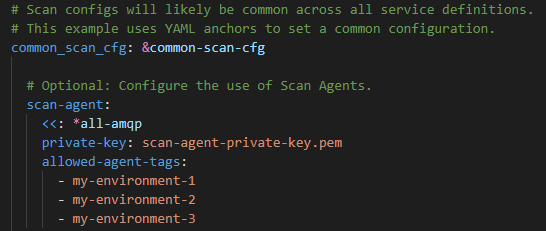
\includegraphics[scale=1]{graphics/scan-agent-config-yaml.png}
    \centering
    \caption{Scan Agent Common Configuration for Server YAML}
    \label{fig:scan-agent-config-yaml}
\end{figure}


\subsection{Message Queue Configuration}

The \cxoneflow endpoint will configure the AMQP Exchanges and Queues upon start.  Adding any
allowed Scan Agent tags will require at least one \cxoneflow endpoint restart so that the
appropriate message queue elements for that tag can be constructed.

The message queue connection credentials for the \cxoneflow endpoint will have the 
permissions required to enable configuring the message queue elements.  Section \ref{sec:external-mq}
will give more details about the appropriate message queue user permissions for the \cxoneflow endpoint.

Configuring a Scan Agent will require each agent to have credentials that allow limited
access to the message queue.  Section \ref{sec:scan-agent-security} has more details about the
authorization that should be assigned to credentials used by Scan Agents.

The YAML examples in \intlink{sec:scan-agent-yaml-config}{the previous section} demonstrated the use of a single
message queue instance for both the communication with the Scan Agents and feedback workflow
orchestration.  While using a single message queue may make the \cxoneflow configuration simpler, it is not
strictly required to use the same message queue connection for all configurations.  Each configuration can
use a segregated message queue server if this is desired.  This segregation includes the use
of \extlink{https://www.rabbitmq.com/docs/vhosts}{virtual hosts} if supported by the AMQP endpoint server.


\subsection{Deployment Considerations}

The YAML examples in \intlink{sec:scan-agent-yaml-config}{Scan Agent configuration section} demonstrated agent tags
configured in a single endpoint service definition.  The allowed tags in each service endpoint are
indicating which agent tags can execute resolver scans and pre-scan scripts for an event handled by that service endpoint.
The tags are used to communicate with Scan Agents that listen for messages directed to that agent tag and
have the public key associated with the private key defined in the service configuration.

The important thing to note is that Scan Agents are not tied to a single
\cxoneflow endpoint service definition.  The Scan Agents will typically have
tooling and configuration that can be used for any code that requires that tooling.  This
has some implications in how Scan Agents can be deployed:

\begin{itemize}
  \item One instance of a Scan Agent can handle multiple tags.
  
  \item More than one instance of a Scan Agent can be deployed to handle the same tag.  This increases the number of concurrently
  executing Scan Agents.

  \item The Scan Agent tag/private key pair can be different in each service definition.  It is recommended to
  use duplicate Scan Agent tags across \cxoneflow service definitions only when those tags all share the same public/private
  key pair.

  \item Not all service definitions need to support the same allowed Scan Agent tags.  If there are Scan Agents
  that should only be used by a specific service definition, it is recommended to use the allowed Scan Agent tag list
  in combination with Scan Agent connection credentials that limit the agent's ability to receive
  communications for specific tags.

  \item For complex \cxoneflow configurations that have many service definitions, it is recommended to engineer
  deployment of Scan Agents to be as simple as possible.
    
\end{itemize}



\section{Distributed Resolver Agent Installation and Configuration}\label{sec:resolver-agent}

\subsection{Overview}

The distributed resolver agent is a service intended to run in a build environment that
matches the build environment generally used for the code.  The service executes
the \scaresolver when events are handled by \cxoneflow that would invoke a scan.
The \scaresolver is typically executed in the code's build pipeline as a pre-step
for a multi-engine \cxone scan that includes an SCA scan.

The keys to a successful \scaresolver scan are generally:

\begin{itemize}
  \item The build tools used to obtain the dependency tree are the same versions and
    configurations as those used to build the code.
  \item The execution happens behind the enterprise firewall to allow for transitive
    dependency resolution of packages that are hosted in a private package repository.
\end{itemize}


\subsection{Installation and Configuration Pre-Requisites}

To install the distributed resolver agent, the following is required:

\begin{itemize}
  \item The distributed resolver agent installer appropriate for your target platform.
  \item An external message queue used by \cxoneflow and the distributed resolver agent (see Section \ref{sec:external-mq} for more details).
  \item A set of message queue credentials used by the distributed resolver agent (see Section \ref{sec:agent-mq-auth-req} for more details).
  \item A public key that is matched with a private key configured for use by the \cxoneflow server (see Section \ref{ref:server-key-pair} for more details).
  \item \scaresolver must be installed if intending to execute \scaresolver without a container.
  \item If intending to execute \scaresolver in a container:
  \begin{itemize}
    \item The system must have docker installed.
    \item The \toolkit build environment must be installed.
  \end{itemize}
\end{itemize}


\subsubsection{Message Queue Authorization}\label{sec:agent-mq-auth-req}

Distributed resolver agents communicate with \cxoneflow using an AMQP message queue. Each distributed
resolver agent must have a set of message queue credentials that limit how it can interact
with the message queue as appropriate for the agent's configured tags.

Table \ref{tab:agent-mq-user-perms} shows the permissions needed for the distributed resolver agent
to interact with the message queues.  Using a regular expression of "\texttt{\^{}cx:res:.*}" will allow
the agent to respond to events for any tag.  It is possible to limit which tags an agent can consume
by adding regular expressions that specify one or more tags at the end of the queue name.  For example, the
regular expression "\texttt{\^{}cx:res:.*(general|java-gradle)\$}" will limit the distributed resolver agent
to handling only tags \texttt{general} and \texttt{java-gradle}.

\begin{table}[ht]
  \caption{RabbitMQ User Permissions for the Distributed Resolver Agent}  
  \label{tab:agent-mq-user-perms}      
  \begin{tabularx}{\textwidth}{lcl}
      \toprule
      \textbf{Permission} & \textbf{Regular Expression} \\
      \midrule
      \texttt{Configure} & blank \\
      \midrule
      \texttt{Write} & \texttt{\^{}cx:res:.*} \\
      \midrule
      \texttt{Read} & \texttt{\^{}cx:res:.*} \\
      \midrule
      \bottomrule
  \end{tabularx}
\end{table}

Table \ref{tab:agent-mq-topic-perms} shows the topic permissions that limit the distributed resolver agent
to submitting messages with topics for scan completion.  Using the regular expression\\"\texttt{\^{}.exec.sca-resolver.scan-complete.*}"
allows the agent to post scan results for any agent.

To limit the agent to submitting messages with only the topics for tags the agent supports, the regular expression can
be modified to include the tags.  For example, the topic regular expression
"\texttt{\^{}.exec.sca-resolver.scan-complete.(general|java-gradle)\$}" will limit the agent to submitting
scan results for the tags \texttt{general} and \texttt{java-gradle}.

\begin{table}[ht]
  \caption{RabbitMQ User Topic Permissions for the Distributed Resolver Agent}  
  \label{tab:agent-mq-topic-perms}      
  \begin{tabularx}{\textwidth}{lcl}
      \toprule
      \textbf{Exchange} & \textbf{Permission} & \textbf{Regular Expression} \\
      \midrule
      \texttt{cx:res:SCA Resolver Scan In} & \texttt{Write} & \texttt{\^{}.exec.sca-resolver.scan-complete.*}\\
      \midrule
      \texttt{cx:res:SCA Resolver Scan In} & \texttt{Read} & blank \\
      \midrule
      \bottomrule
  \end{tabularx}
\end{table}

\subsubsection{Distributed Resolver Agent Deployment Considerations}

The \cxoneflow scan workflow that delegates resolver scans to distributed resolver agents
assumes that one or more agents are available to handle the delegated scan request. Any number
of distributed resolver agents that handle the same tag can be deployed.  It is suggested that
deployment of distributed resolver agents considers that resolver scans will fail in the event
that no distributed resolver agents are available to handle scan requests for one or more
tags.


\subsection{Security Considerations}\label{sec:resolver-agent-security}

As briefly described in Section \ref{sec:dist-resolver-security-considerations}, executing
part of a code build to extract a dependency tree can pose some risks. For example,
tools like Gradle define the build definition in the programming language Groovy; this Groovy
code executes when Gradle loads the build definition.  Other tools even execute scripts defined
in the dependency package leading to the popular method of "typo-squatting" as a means to
perform a remote-code-execution (RCE) attack directly on unsuspecting developers.  Executing an
untrusted build definition or loading a dependency containing malware into a build system is
a risk that comes from using open-source software.

Since the risk of malicious builds is always possible, the deployment of the distributed resolver agent
can be configured to mitigate these risks.  The section for each platform's install makes specific
recommendations for a secure deployment of the distributed resolver agent.  The general recommendations
for all platform deployments are:

\begin{itemize}
  \item \textbf{Assume that anyone with administrative access to a server with a distributed resolver agent installed
    can intercept all secrets configured on the \cxoneflow server.}
  \item It is a best practice to not allow developers administrative control over the configuration and
    execution of the distributed resolver agent.
  \item Utilize file permissions on the secret values used by the agent to limit which running processes
    can read the contents of the secrets
  \item Use the recommended file system permissions for each platform's deployment.
  \item Find a logical grouping of agents for message queue credential assignment to better avoid
    impact if any credentials are misused.
  \item Use the message queue account security settings to limit message queue access to agents such that they are only
    able to receive and send events required for their specific operations.
  \item If the agent is invoking \scaresolver as a shell execution, utilize a "run-as" configuration to
    run the resolver as a low-privilege account.
  \item Utilize the \scaresolver docker execution capability to sandbox the dependency resolution in a container.
  \item Avoid configuring a distributed resolver agent instance to execute \scaresolver for both shell and container dependency resolution
    unless proper precautions have been taken to avoid privilege escalation exploits through the container file system overlay.
\end{itemize}



\subsubsection{Installing on Debian Linux}

The installation on Debian Linux platforms uses the distributed resolver agent Debian installer package
found with the \cxoneflow release.  The installer performs the following steps:

\begin{itemize}
  \item The agent is installed at the path \texttt{/opt/cxoneflow-resolver-agent}
  \item The agent uses the configuration file \texttt{/etc/cxoneflow-resolver-agent/config.yaml}
  \item A config template is installed at \texttt{/etc/cxoneflow-resolver-agent/config.template.yaml}
  \item The agent is installed as a \texttt{systemd} service and registered to automatically run at system start.
  \item The non-login user \texttt{resolver} is created and used to execute the \texttt{systemd} service.
  \item The non-login user \texttt{resolver-runtime} is created for use with the optional run-as isolation
    (see \intlink{par:shell-agent-isolation}{Shell Execution Isolation} for this optional configuration).
  \item A default directory for storing secrets is created at \texttt{/var/secrets} with permissions 500.
\end{itemize}

As part of the configuration, a work directory for the resolver will be required.  When this directory
is created, it is recommended to use the owner of \texttt{root:resolver} and permissions of 770.  This
directory will primarily store temporary files used during the execution of \scaresolver.

The default secrets directory \texttt{/var/secrets} is created with ownership \texttt{resolver:resolver} and
permissions 500.  For secret files placed in this directory, it is recommended to each file is owned
by \texttt{resolver:resolver} with permissions of 400.  The permission of 400 will prevent 
build tools from reading the secrets when using the \intlink{par:shell-agent-isolation}{Shell Execution Isolation} option.

\paragraph{Controlling the Distributed Resolver Agent}
\noindent\\The distributed resolver agent runs as a \texttt{systemd} service.  This allows the run status to be controlled
by commands such as "\texttt{systemctl start cxoneflow-resolver-agent}" and\\"\texttt{systemctl stop cxoneflow-resolver-agent}".

The distributed resolver agent runtime logs appear in \texttt{/var/log/syslog}.  To monitor the distributed resolver agent logs, execute the command
\\"\texttt{tail -f /var/log/syslog | grep resolver.agent}".

Debug logging can be turned on for the distributed resolver agent by adding an environment variable in the \texttt{systemd}
service definition.  The following procedure will enable debug logging:

\begin{enumerate}
  \item Edit the file \texttt{/opt/cxoneflow-resolver-agent/cxoneflow-resolver-agent.service}
  \item Add the line "\texttt{Environment=LOG\_LEVEL=DEBUG}" under the existing line starting with\\\texttt{Environment}.
  \item Save the modifications to the \texttt{cxoneflow-resolver-agent.service} file.
  \item Execute the command "\texttt{systemctl daemon-reload}".
  \item Execute the command "\texttt{systemctl restart cxoneflow-resolver-agent}".
\end{enumerate}

\paragraph{Shell Execution}\label{par:agent-shell-execution}

\noindent\\Shell execution of \scaresolver is configured to use an instance of \scaresolver installed on the local system.
The execution of \scaresolverns, along with all build tools it invokes as part of the scan are executed with the \texttt{resolver}
user.  The \texttt{resolver} user is the executing user since the process is spawned from the \texttt{systemd} service that also
runs as the \texttt{resolver} user.

The \texttt{resolver} user is a non-login user that should have no access to do much other than run \texttt{git}, \scaresolverns, and
the build tools invoked as part of the dependency resolution.  The home directory for the \texttt{resolver} user is dynamically set
to the value configured in \intlink{sec:agent-resolver-work-path}{resolver-work-path} when \scaresolver is executed.  The location
of the home directory may have implications for how the build tools run.

Many build tools will have several places where they will look for configurations that are not explicitly placed in the build
definition.  In some cases, the configuration can exist in the home directory of the user running the build tool.  It may be necessary
to replicate build tool settings to the \intlink{sec:agent-resolver-work-path}{resolver-work-path}.  If the build tools use a global location
for the settings, it may be necessary to adjust file/directory permissions to allow the \texttt{resolver} user to access the global
configurations.

The build tools will often use the running user's home directory to write a package cache.  When the tool is invoked,
the running user's home directory is set to the value configured in \intlink{sec:agent-resolver-work-path}{resolver-work-path}.
It may be possible to change the locations where the tools look for configuration or write package caches by configuring the
\intlink{sec:agent-resolver-opts}{resolver-opts} YAML element with
\extlink{https://docs.checkmarx.com/en/34965-132888-checkmarx-sca-resolver-configuration-arguments.html\#UUID-bc93274b-c1c7-ea47-9556-3bd8900711dc_id_CheckmarxSCAResolverConfigurationArguments-CustomParameters}
{custom parameters} passed to the build tools.

If transitioning to a configuration for \intlink{par:shell-agent-isolation}{Shell Execution Isolation}, the contents of the directory
defined in \intlink{sec:agent-resolver-work-path}{resolver-work-path} will be owned by \texttt{resolver:resolver}.  This will likely
cause \scaresolver to fail since the change in configuration will cause the user running the tools to change to
\texttt{resolver-runtime}.  Most of the tools will require files and directories to be owned by\\\texttt{resolver-runtime:resolver}.
It may be necessary to purge the \intlink{sec:agent-resolver-work-path}{resolver-work-path} directory or selectively change
the ownership of build-tool related files/directories to \texttt{resolver-runtime:resolver}.


\subparagraph{Shell Execution Isolation}\label{par:shell-agent-isolation}
\noindent\\Using the shell execution isolation configuration is an advanced option that requires granting limited sudoer privileges
to the \texttt{resolver} user.  The sudoer privileges required are to allow the \texttt{resolver} user to execute \scaresolver
as the user configured in \intlink{sec:agent-resolver-run-as}{resolver-run-as}.  The reason to use this option is to ensure that
the contents of the files located in the \intlink{sec:yaml-secret-root-path}{secret-root-path} can't be read while \scaresolver
is executing.\footnote{This assumes the recommendation of setting the permissions of each file in 
\intlink{sec:yaml-secret-root-path}{secret-root-path} to 400 has been followed.}

The installer creates a no-login user \texttt{resolver-runtime} as a default user that can be referenced in the \intlink{sec:agent-resolver-run-as}{resolver-run-as}
configuration.  Another user can be used as long as the primary group membership is the \texttt{resolver} group.  In most configurations, 
the \texttt{resolver-runtime} user will be sufficient.

The package installer does not configure this user with sudoer privileges by default primarily since the location of the \scaresolver
installation is unknown.  It is also best to allow a system administrator to be explicitly aware of users with sudoer privileges when installing
package.

To enable the \texttt{resolver-runtime} user to have the required privileges, the following procedure can be followed:

\begin{enumerate}
  \item Execute the command "\texttt{visudo /etc/sudoers.d/00-resolver}".
  \item Add the single line:\\"\texttt{resolver ALL=(resolver-runtime) NOPASSWD: SETENV: /path/to/ScaResolver}"
  \item Save the \texttt{/etc/sudoers.d/00-resolver} file.
  \item Configure the element \intlink{sec:agent-resolver-run-as}{resolver-run-as} in \texttt{/etc/cxoneflow-resolver-agent/config.yaml} 
  with the user \texttt{resolver-runtime}.
  \item Restart the \texttt{systemd} service for the distributed resolver agent.
\end{enumerate}

Any configuration for tags that use shell execution of \scaresolver will now run as the user\\\texttt{resolver-runtime}.

\paragraph{Container Execution}
\noindent\\Container execution is supported using the \toolkit build environment that will extend a container image
specified in the \intlink{sec:agent-container-image-tag}{container-image-tag} YAML element.  The extended image
installs \scaresolver at the \texttt{systemd} service start.

The execution of \scaresolver is isolated from the underlying operating system by executing in the container image.
The container image, having all appropriate build tools and build tool configuration, will perform a dependency
tree resolution in the same way as it is done with shell execution.  This is similar to using
\intlink{par:shell-agent-isolation}{Shell Execution Isolation} by delegating execution to the docker image.

Assuming \texttt{docker} is installed, it is generally required to add the \texttt{resolver} user to the \texttt{docker}
group using the command "\texttt{usermod -a -G docker resolver}".  This allows the \texttt{resolver} user to execute
commands to build and run containers.

\subparagraph{Container Execution Security}
\noindent\\The installation of \texttt{docker} is usually done such that the \texttt{docker} daemon runs with
root privileges.  For distributed resolver agent configurations that allow 
\intlink{par:agent-shell-execution}{Shell Execution} along with container execution, this capability could pose
the risk of privilege escalation via the \texttt{docker} runtime.

If not configured for \intlink{par:shell-agent-isolation}{Shell Execution Isolation}, it is possible that
executing build tools via \scaresolver running as the \texttt{resolver} user can escalate privileges
to read and write files with root privileges.  This is due to the \texttt{resolver} user being a member of
the \texttt{docker} group and \scaresolver executing as \texttt{resolver}.  

To avoid the potential for privilege escalation:

\begin{itemize}
  \item Use \intlink{par:shell-agent-isolation}{Shell Execution Isolation} for distributed resolver agents that are configured
    to execute \scaresolver both as a shell execution and using container execution.
  \item If not using \intlink{par:shell-agent-isolation}{Shell Execution Isolation}, install \texttt{docker} in the "rootless"
    configuration.\footnote{As of the writing of this manual, this is not a tested configuration scenario.  It is unknown if rootless will work.
    An alternative would be to avoid configurations that allow both shell and docker execution of \scaresolverns.}
\end{itemize}



\subsection{Distributed Resolver Agent YAML Configuration}

The distributed resolver agent's YAML configuration is deployed after the agent is installed.
Many of the elements share format with the \intlink{sec:yaml-config}{server's configuration elements}. 


Figure \ref{fig:resolver-agent-config-yaml} shows an example of the serviced tag configurations for 
a distributed agent YAML configuration.  The example YAML can be downloaded from the \cxoneflow YAML
example release artifacts.

\begin{figure}[h]
    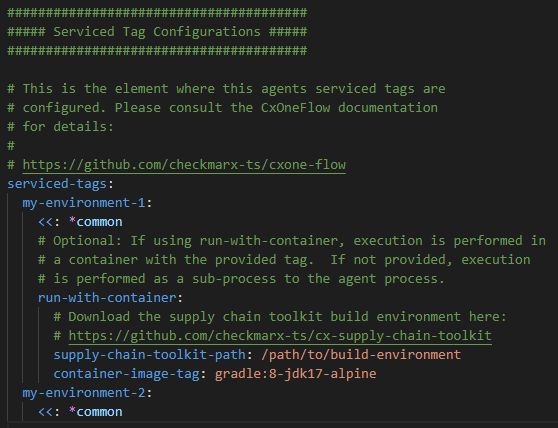
\includegraphics[width=\textwidth]{graphics/resolver-agent-config-yaml.png}
    \caption{Distributed Resolver Agent Configuration YAML}
    \label{fig:resolver-agent-config-yaml}
\end{figure}

\pagebreak

\subsubsection{Distributed Resolver Agent YAML Configuration Tree}\label{sec:agent-yaml-root}

\dirtree{%
    .1 <root>.
    .2 \intlink{sec:yaml-secret-root-path}{secret-root-path}\DTcomment{[Required]}.
    .2 \intlink{sec:agent-serviced-tags}{serviced-tags}\DTcomment{[Required]}.
    .3 \intlink{sec:agent-tag}{<agent tag>}\DTcomment{[At least 1 required]}.
    .4 \intlink{sec:yaml-generic-amqp}{amqp}\DTcomment{[Optional] Default: localhost}.
    .5 \intlink{sec:yaml-generic-amqp-amqp-password}{amqp-password}\DTcomment{[Optional]}.
    .5 \intlink{sec:yaml-generic-amqp-amqp-url}{amqp-url}\DTcomment{[Required]}.
    .5 \intlink{sec:yaml-generic-amqp-amqp-user}{amqp-user}\DTcomment{[Optional]}.
    .5 \intlink{sec:yaml-generic-ssl-verify}{ssl-verify}\DTcomment{[Optional] Default: True}.
    .4 \intlink{sec:agent-public-key}{public-key}\DTcomment{[Required]}.
    .4 \intlink{sec:agent-resolver-opts}{resolver-opts}\DTcomment{[Optional] Default: None}.
    .4 \intlink{sec:agent-resolver-path}{resolver-path}\DTcomment{[Required if not \texttt{run-with-container}]}.
    .4 \intlink{sec:agent-resolver-run-as}{resolver-run-as}\DTcomment{[Optional] Default: run as service user}.
    .4 \intlink{sec:agent-resolver-work-path}{resolver-work-path}\DTcomment{[Optional] Default: /tmp/resolver}.
    .4 \intlink{sec:agent-run-with-container}{run-with-container}\DTcomment{[Required if not \texttt{resolver-path}]}.
    .5 \intlink{sec:agent-container-image-tag}{container-image-tag}\DTcomment{[Required]}.
    .5 \intlink{sec:agent-supply-chain-toolkit-path}{supply-chain-toolkit-path}\DTcomment{[Required]}.
    .5 \intlink{sec:agent-use-running}{use-running-gid}\DTcomment{[Optional] Default: True}.
    .5 \intlink{sec:agent-use-running}{use-running-uid}\DTcomment{[Optional] Default: True}.
}

\input{resolver/yaml/root.tex}
\input{resolver/yaml/serviced-tags.tex}
\subsubsection{<agent tag>.disable-resolver}\label{sec:agent-disable-resolver}
Defaults to \texttt{False}.  Set to \texttt{True} to disable execution of \scaresolver.  This is typically used with 
\intlink{sec:agent-pre-scan}{pre-scan} configured to execute a scan step that does not require the use of \scaresolver.

If this is set to \texttt{True}, options \intlink{sec:agent-resolver-path}{resolver-path} and 
\intlink{sec:agent-run-with-container}{run-with-container} are ignored.


\subsubsection{<agent tag>.pre-scan}\label{sec:agent-pre-scan}
This element contains elements to support \intlink{sec:scan-agent-prescan}{pre-scan scripting}.

\subsubsection{<agent tag>.pre-scan.container-image-tag}\label{sec:agent-pre-scan-container-image-tag}
This is a tag to a container image where the configured \intlink{sec:scan-agent-prescan}{script} will execute.

\subsubsection{<agent tag>.pre-scan.resolver-before-script}\label{sec:agent-pre-scan-resolver-before-script}
If set to \texttt{False} (the default), \scaresolver executes after the \intlink{sec:agent-pre-scan-script}{pre-scan script}.
If set to \texttt{True}, \scaresolver executes before the \intlink{sec:agent-pre-scan-script}{pre-scan script}. If \scaresolver
execution has been disabled with the \intlink{sec:agent-disable-resolver}{disable-resolver} option, this setting is ignored.


\subsubsection{<agent tag>.pre-scan.run-as-agent}\label{sec:agent-pre-scan-run-as-agent}
The default setting is \texttt{True}.  If set to \texttt{True}, the container runs with the UID:GID of
the scan agent.  This is to allow for the overlay file system to read/write to the mapped code directory
while executing the pre-scan script.  If set to \texttt{False}, the container runs as the container default
user.

When running as the container default user, anything written to the mapped code directory may prevent the scan
agent from having read/write access after the container exits.  The pre-scan script should set the read/write
permissions on or remove files written during the container execution prior to exiting the container.  This will
allow the scan agent to remove the temporary copy of the code when the pre-scan execution is complete.


\subsubsection{<agent tag>.pre-scan.script}\label{sec:agent-pre-scan-script}
The script to execute in the running container image.  This can be a single line or a multi-line
string using the \extlink{https://yaml.org/spec/1.2.2/\#812-literal-style}{YAML literal scalar style} syntax
by using the bar character ("\texttt{|}") as the value and indenting the next several lines to form the
complete script.


\subsubsection{<agent tag>.pre-scan.shell}\label{sec:agent-pre-scan-shell}
By default, the pre-scan script will execute in the container's shell located at \texttt{/bin/sh}.  This is a standard shell location
in most Linux distributions.  The path to an alternate shell on the container image can optionally be defined here.

\subsubsection{<agent tag>.public-key}\label{sec:agent-public-key}
The value specifies a file name found under the path defined by \texttt{secret-root-path} containing a 
public key that matches the server's configured \intlink{sec:yaml-resolver-private-key}{\texttt{private-key}} setting.


\subsubsection{<agent tag>.resolver-opts}\label{sec:agent-resolver-opts}
This is a dictionary of
\extlink{https://docs.checkmarx.com/en/34965-132888-checkmarx-sca-resolver-configuration-arguments.html\#UUID-bc93274b-c1c7-ea47-9556-3bd8900711dc_id_CheckmarxSCAResolverConfigurationArguments-ConfigurationArguments-TablesandSamples}{configuration arguments}
passed to \scaresolver when executing.  The options are used to provide static values for resolver execution configuration.  Some of the
options may clash with execution options provided by the agent; options that would clash with how the agent executes \scaresolver are ignored.  

The \texttt{resolver-opts} section is a dictionary of key and key/value pairs that correspond to
\extlink{https://docs.checkmarx.com/en/34965-132888-checkmarx-sca-resolver-configuration-arguments.html}{command line options} for \scaresolver.
The options that can be used are limited considering some of the options are used by the \cxoneflow integration to execute \scaresolver.

These options, if set, will be ignored:

\begin{itemize}
  \item logs-path
  \item a | account
  \item containers-result-path
  \item resolver-result-path
  \item project-name
  \item authentication-server-url
  \item p | password
  \item sso-provider
  \item sca-app-url
  \item s | scan-path
  \item server-url
  \item u | username
  \item project-tags
  \item scan-tags
  \item bypass-exitcode
  \item no-upload-manifest
  \item help
  \item manifests-path
  \item t | project-teams
  \item q | quiet
  \item save-evidence-path
  \item severity-threshold
  \item report-content
  \item report-extension
  \item report-path
  \item report-type
  \item sast-result-path
  \item cxpassword
  \item cxuser
  \item cxprojectid
  \item cxprojectname
  \item cxserver
\end{itemize}

\subsubsection{<agent tag>.resolver-path}\label{sec:agent-resolver-path}
The path to the \scaresolver executable that has been installed on the system running the Scan Agent.


\subsubsection{<agent tag>.resolver-run-as}\label{sec:agent-resolver-run-as}
The name of a user account that will run the \scaresolver when executed in a shell (but not as a container).  This
is an advanced configuration that will require additional configuration for your platform.  

If not provided, the \scaresolver is executed as the same user that is running the Scan Agent service.

\subsubsection{<agent tag>.scan-agent-work-path}\label{sec:scan-agent-work-path}
A path where temporary files are written during the operation of the Scan Agent.  This also serves as the home
directory for the Scan Agent user and the user defined in \texttt{resolver-run-as}.

\subsubsection{<agent tag>.run-with-container}\label{sec:agent-run-with-container}
A YAML dictionary with key/value pairs used to define running \scaresolver in a container.  If this is supplied,
the configured \texttt{resolver-path} is ignored and \scaresolver will not be invoked in a shell.  The dependency
tree collected by \scaresolver will be done by executing build tools defined in the container.  This is useful for
organizations that utilize containerized build environments in their CI/CD pipeline build scripts.

The use of containers to run \scaresolver is not supported on Windows platforms.

\subsubsection{<agent tag>.run-with-container.container-image-tag}\label{sec:agent-container-image-tag}
The container tag that is found in one of the logged-in container registries.  This container tag is used by the \toolkit
to create an extended image with \scaresolver installed.

\subsubsection{<agent tag>.run-with-container.supply-chain-toolkit-path}\label{sec:agent-supply-chain-toolkit-path}
The path where the \toolkit build environment is installed.

\subsubsection{<agent tag>.run-with-container.use-running-gid and\\<agent tag>.run-with-container.use-running-uid}\label{sec:agent-use-running}
These options are True by default.  This causes the image built by the \toolkit to use the
UID and primary GID of the user running the Scan Agent when defining a non-root
user in the extended image.  

The reason for this is that when \scaresolver is executed in the container, temporary paths
in the \texttt{resolver-work-path} are mapped to the container.  Files created by the container
will have the UID/GID of the running container's user when created.  Since the UID/GID of the
container matches the UID/GID of the Scan Agent, the files that remain after
the container exits can be controlled by the Scan Agent.

Setting these values to False should only be done in circumstances where the UID/GID for written files
should be defined by the container.  This scenario may never practically exist.



\subsection{Resolver Configuration Recommendations}

The YAML configuration option \intlink{sec:agent-resolver-opts}{resolver-opts} can be used to provide
configuration options for \scaresolver during execution.  This section discusses recommended
configuration options.

\subsubsection{break-on-manifest-failure}\label{sec:break-manifest}

This is a boolean option that is passed to \scaresolver as the argument \texttt{--break-on-manifest-failure}.  It is recommended
that this is set in the \intlink{sec:agent-resolver-opts}{resolver-opts} configuration.  This will cause any manifest failures
encountered when running \scaresolver to flag the scan with the resolver tag of \textbf{failed}.  If this option is not included,
all scans will have a resolver tag of \textbf{success} regardless of if resoluton of any dependency trees failed when
executing \scaresolverns.

The reason \scaresolver should be configured to run with this option is to make it easy to filter a list of scans by resolver
failure status.  All SCA scans are reported as successfully completed if the dependency tree resolution executes to
any type of completion.  The dependency resolution may completely or partially fail but the scan status will reflect
as a successful scan.  Any partial results will be reported but it requires some manual review of logs to understand if there
were any partial dependency tree resolution failures.

\subsubsection{scan-containers}
This is a boolean option that is passed to \scaresolver as the argument \texttt{--scan-containers}.  It is recommended that
this option is \textbf{not} set in the \intlink{sec:agent-resolver-opts}{resolver-opts} configuration.

There are a few reasons for omitting this flag; the main reason is that container security scans have moved away from
using \scaresolver to perform the scan.  Container security scans are now an independent scan option and no longer
report results provided by \scaresolver when used by \cxonens.  This option may remain in \scaresolver for backwards
compatibility with other Checkmarx products.

\subsection{Limitations}
Please note the following limitations apply when using the distributed resolver agent:

\begin{itemize}
  \item Server-side configurations with \texttt{clone-auth} using SSH keys will fail.
  \item Windows base container images can not be used to run \scaresolver in a container.  Only Linux base images are supported.
  \item The Containter Security scans recently moved away from using \scaresolverns, thus container scans will currently
    execute in the \cxoneflow server side environment.
\end{itemize}



